\documentclass{article}

\usepackage{physics}
\usepackage{siunitx}
\usepackage{amsmath}
\usepackage{tikz}
\usepackage{graphicx}

\graphicspath{{./figs/}}


\title{Simulation of time dependent hamiltonian}
\author{Martin Johnsrud}
\date{}

\begin{document}

\maketitle

\section*{Parametres}

    The 1D time dependent Schrödinger equation is given by

    \begin{equation*}
        \hat H \Psi(x, t) = i \hbar \pdv{t} \Psi(x, t), \quad \hat H = -\frac{\hbar}{2m}\pdv[2]{x} + V(x, t),
    \end{equation*}

    for some potential $V(x)$. However, it is cumbersom to walk with dimensonfull constants, especially numerically, when values for $\hbar$ in the si-system is of order $10^{-34}$. This can lead to inaccuracies when doing numerical simulations. But, by choosing some defining, problem-dependent sizes and grouping togheter the constants, this can be liminated by the introduction of dimensonless variables. We are going to be working with potentials which are infinit outside som local region, i.e. the boundary conditions $\psi(0>x>L) = 0$, so it is natural to choose the length of the potential, $L$, as a defining quantity. Noticing that

    \begin{equation*}
        \bigg[\frac{\hbar}{2 m L^2} \bigg] = \frac{\si{kg.m^2.s^{-1}}}{\si{kg.m^2}} = \si{s^{-1}},
    \end{equation*}
    we make the variable change
    \begin{equation*}
        \frac{\hbar}{2 m L^2}t \rightarrow t, \quad \frac{1}{L}x \rightarrow x.
    \end{equation*}
    This gives the new, dimensionless schrödinger equation
    \begin{equation}
        \hat H \Psi(x, t) = -i \pdv{t} \Psi(x, t), \quad \hat H = -\pdv[2]{x} + V(x, t),
        \label{time_depend}
    \end{equation}
    where I have done the change $2mL/\hbar^2V(x, t) \rightarrow V(x, t)$. All sizes now is in units defined by the problem and the constants of the equation, and the new boundary condition is 
    \begin{equation*}
        \Psi(0>x>1) = 0.
    \end{equation*}

    \section*{Time independent problems}
    Assuming, for now, that the potential is independent of time, we can get the time independent schrødinger equation from \eqref{time_depend} by separation of variables. Assuming $\Psi(x, t) = \psi(x)\phi(t)$  yields the time independent schrödinger equation and the equation for the time dependence:
    \begin{equation}
        \bigg[-\pdv[2]{x} + V(x) \bigg] \psi(x) = \hat H \psi = E \psi(x), \quad \pdv{t}\phi(t) = -iE\phi(t).
    \end{equation}
    The equation for time is elematary, and gives the solution
    \begin{equation*}
        \phi(t) = \exp(-iEt).
    \end{equation*}
    The time independent schrödinger equation is a eigenvalue problem, and can be solved by discretizing the hamiltonian, and thus also $\psi$. We are first going to look at a particle in a box, i.e. $V(0<x<1) = 0$. The euqaion to discretize is thus
    \begin{equation*}
        \pdv[2]{x}\psi(x) = E \psi(x).
    \end{equation*}
    Using a finite difference scheme with $N + 1$ nodes, there will be $N-1$ possibly non-zero nodes. The end node are given by the boundary conditions $\psi(0) = \psi(1) = 0$, and the interior points are given by the matrix equation
    \begin{equation*}
        D \psi_n = E_n \psi_n, \quad D_{ii} = 2N^2, D_{ii\pm1} = -N^2.
    \end{equation*}
    Here, $\psi_n$ is a vector such that $\psi_n^{(j)} = \psi_n\big((j+1)/N\big)$. This is shown in the figure below.

    \vspace{10pt}
    {\centering
    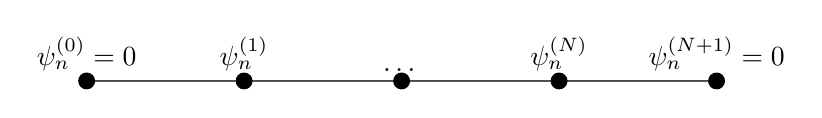
\begin{tikzpicture}
        \filldraw
        (0, 0) circle (0.1) node[align=center, above] {$\psi_n^{(0)} = 0$}--
        (2, 0) circle (0.1) node[align=center, above] {$\psi_n^{(1)}$}--
        (4, 0) circle (0.1) node[align=center, above] {\dots} --
        (6, 0) circle (0.1) node[align=center, above] {$\psi_n^{(N)}$}--
        (8, 0) circle (0.1) node[align=center, above] {$\psi_n^{(N+1)} = 0$};
    \end{tikzpicture}
    }
    \vspace{10pt}

    The result of the simulation, togheter with the analytical solution, is shown in figure \ref{fig:particel in box}. The normalization is such that the sum ${\psi_n^{j}}^\dagger\psi_n^{j} = 1$ holds. The analytical solution for the eiegenvalues are $E_n = (n \pi)^2$. By the finite nature of this simulation, the values are going to be less accurate for the higher energies, as they are waves where the wave length is short, and is aproaching the resolution of the discretization. Figure \ref{eigenvalues} shows the numerically computed eigenvalues, and compares them to the analytical solution. We see the error always wil increas rapidly for higher values, but we also get rapidly more accurate values by increasing $N$, i.e. decreasing the steplenght $\Delta x = 1 / N$. In figure \ref{errors}, we can se the trend of the error as the stepsize decrease. It is evident that the error decreases as the square of the steplength, or the inverse of the square of the number of points.

    \begin{figure}[h]
        \centering
        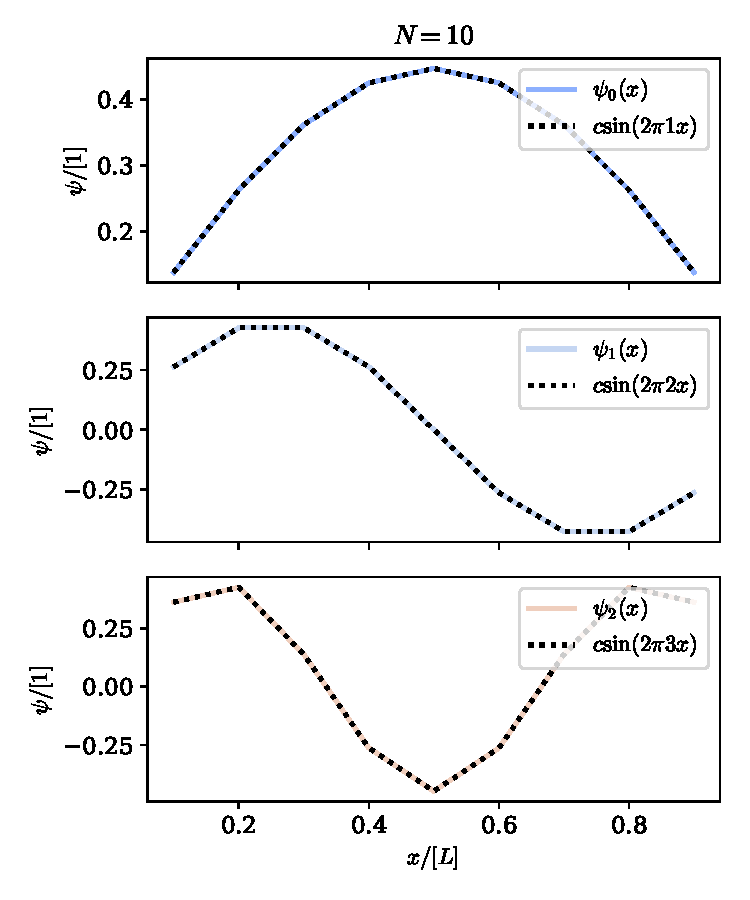
\includegraphics[width=0.49\textwidth]{particle_in_box/vector_N=10}
        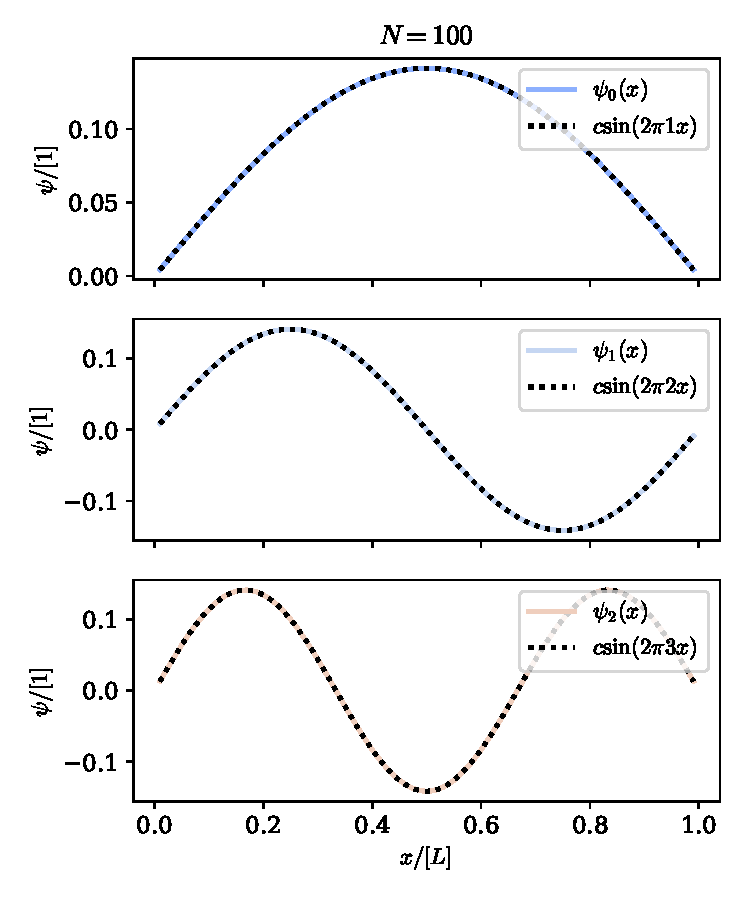
\includegraphics[width=0.49\textwidth]{particle_in_box/vector_N=100}
        \caption{The numerical simulation and analytical solution to a prticle in a box}
        \label{fig:particel in box}
    \end{figure}

    \begin{figure}[h]
        \centering
        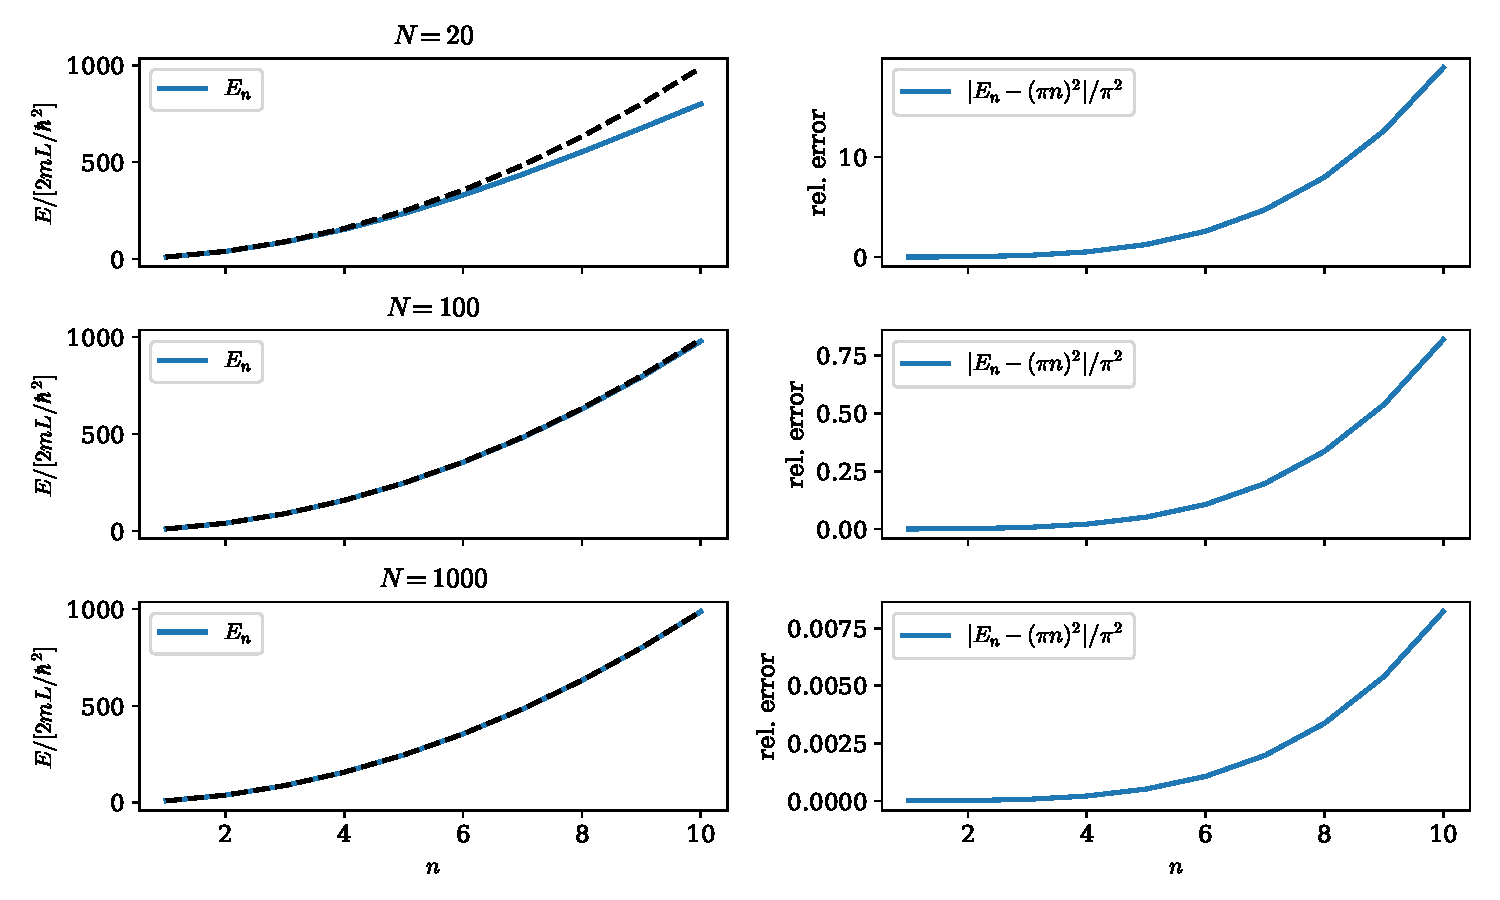
\includegraphics[width=\textwidth]{particle_in_box/values}
        \caption{The numerical eigenvalues, compared with the analytical solution.}
        \label{eigenvalues}
    \end{figure}

    \begin{figure}[h]
        \centering
        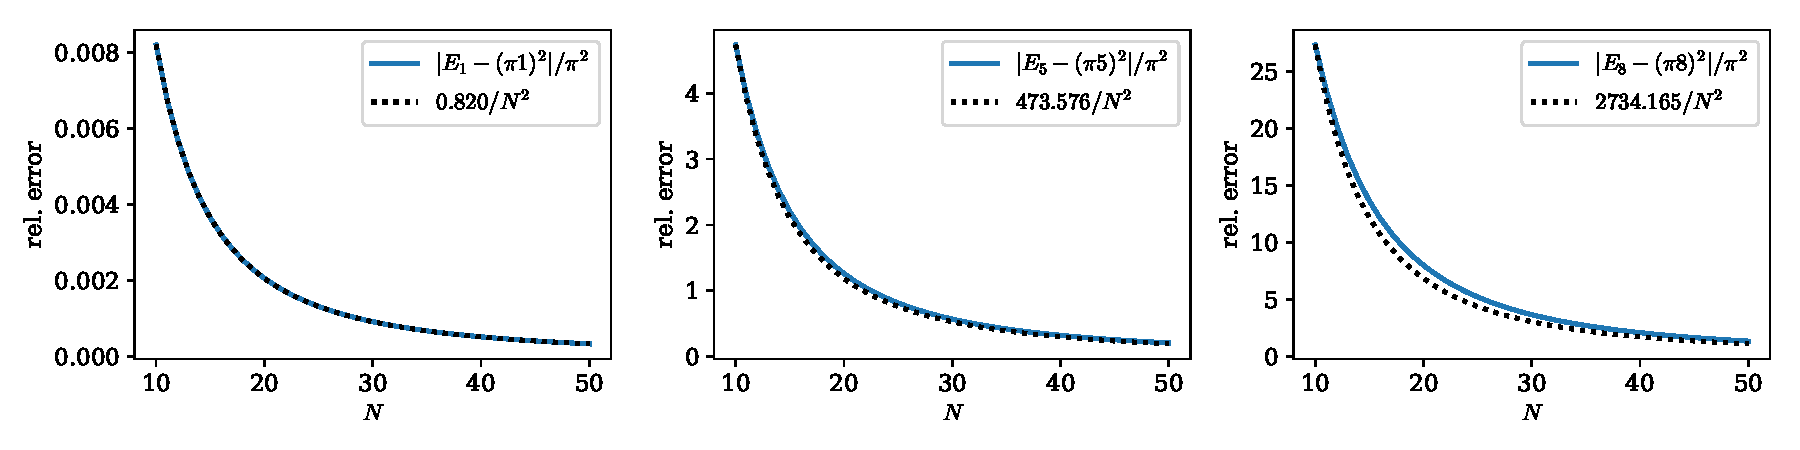
\includegraphics[width = \textwidth]{particle_in_box/error}
        \caption{The errors for some of the few first eigenvalues, compared to the square of the steplength}
        \label{errors}
    \end{figure}

\end{document}